\documentclass[tikz]{standalone}

\usetikzlibrary{matrix,positioning}
\begin{document}

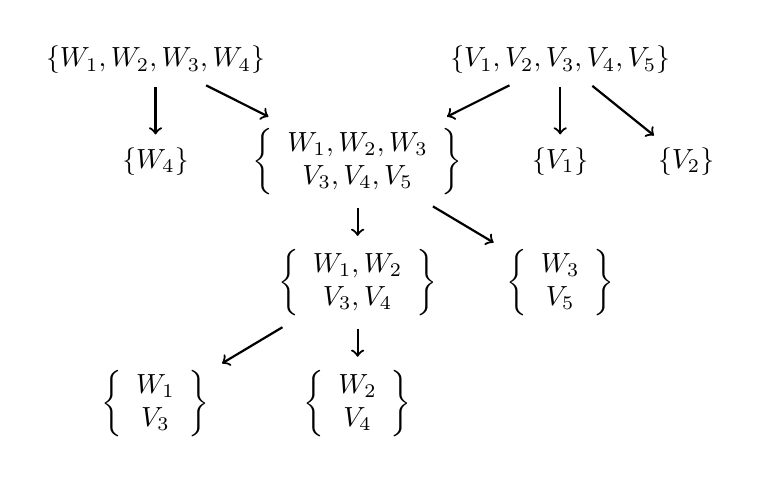
\begin{tikzpicture}[thick,shorten >=1pt, shorten <=1pt,->]
%  \matrix (m) [matrix of math nodes, row sep=3em, column sep={5em,between origins}]{
  \matrix (m) [matrix of math nodes, row sep=1.3em, column sep=-1.1em]{
	 \{W_1,W_2,W_3,W_4\} & & \{V_1,V_2,V_3,V_4,V_5\} & \\
	\{W_4\} & \left\{ \begin{array}{c} W_1,W_2,W_3 \\ V_3,V_4,V_5 \end{array} \right\} & \{V_1\} & \{V_2\} \\
	& \left\{\begin{array}{c} W_1,W_2 \\ V_3,V_4 \end{array}\right\} & \left\{ \begin{array}{c} W_3 \\ V_5 \end{array} \right\}\\
	\left\{ \begin{array}{c} W_1 \\ V_3 \end{array} \right\}  & \left\{ \begin{array}{c} W_2 \\ V_4 \end{array} \right\} & \\
  };
  \path 
  	(m-1-1) edge (m-2-1)
  	(m-1-1) edge (m-2-2)
  	(m-1-3) edge (m-2-2)
  	(m-1-3) edge (m-2-3)
  	(m-1-3) edge (m-2-4)
  	(m-2-2) edge (m-3-2)
  	(m-2-2) edge (m-3-3)
  	(m-3-2) edge (m-4-1)
  	(m-3-2) edge (m-4-2)
  ;
\end{tikzpicture}
\end{document}